%%%%%%%%%%%%%%%%%%%%%%%%%%%%%%%%%%%%%%%%%%%%%%%%%%%%
%%% Standalone Vietnamese sample: Chapter 18
%%%%%%%%%%%%%%%%%%%%%%%%%%%%%%%%%%%%%%%%%%%%%%%%%%%%

\documentclass[output=book,
  colorlinks,citecolor=brown
]{langscibook}

\author{Brett Reynolds}
\title{Cảnh quan ngôn ngữ: Language Landscapes}
\subtitle{Hướng dẫn về cấu trúc tiếng Anh cho giáo viên tiếng Anh [Bản tiếng Việt]}
% \ISBNdigital{}
% \ISBNhardcover{}
% \BookDOI{}
\typesetter{Brett Reynolds}
% \proofreader{}
% \lsCoverTitleSizes{51.5pt}{17pt}
\renewcommand{\lsSeries}{tbls}
%\newcommand{\lsSeriesTitle}{Textbooks in Language Sciences}
%\newcommand{\lsSeriesColor}{lsYellow}
\renewcommand{\lsSeriesNumber}{16}
\BackBody{Ngôn ngữ không phải là một danh sách để học thuộc; đó là một cảnh quan để khảo sát.

Một nhà tự nhiên học giỏi ngoài thực địa không chỉ đặt tên cho sự vật. Họ quan sát chúng vận hành như thế nào, tụ lại ở đâu, và vì sao biến đổi. Cuốn sách này mời bạn đọc tiếng Anh theo cùng cách ấy: chú ý đến những gì người nói thật sự làm, chứ không chỉ những gì sách quy tắc bảo rằng họ nên làm. Khung phân tích dựa trên \textit{The Cambridge Grammar of the English Language}, được trình bày giản lược cho dễ tiếp cận nhưng không hạ thấp mức độ chính xác.

Các chương đi từ âm thanh và từ ngữ đến cụm từ, mệnh đề, rồi diễn ngôn, với những ví dụ tiếng Anh rõ ràng đặt cạnh các lát cắt nhỏ từ những ngôn ngữ khác. Mỗi chương luyện cùng một thao tác: quan sát một khuôn mẫu, kiểm tra nó bằng bằng chứng, nhận ra nơi khuôn mẫu ấy vỡ ra, rồi hỏi sự vỡ ra ấy dạy ta điều gì. Đến cuối sách, bạn sẽ có một vốn ngữ pháp thực dụng đủ sức bảo vệ các nhận định của mình: dùng để đánh giá sách giáo khoa, giải thích vì sao câu của người học nghe chưa ổn, và bảo vệ lời giải thích khi bị chất vấn.

Dù bạn đang trong chương trình đào tạo giáo viên hay đã đứng lớp, lợi ích vẫn như nhau: ngừng dựa vào những quy tắc không thể biện minh, và bắt đầu tự mình nhìn thấy hệ thống của ngôn ngữ.}

\usepackage{langsci-optional}
\usepackage{langsci-gb4e}
\usepackage{langsci-lgr}

% Load xeCJK for Japanese text (needed for マクドナルド etc)
\usepackage{xeCJK}
% Try common CJK serif fonts to match book's serif style
\IfFontExistsTF{Noto Serif CJK JP}{
  \setCJKmainfont{Noto Serif CJK JP}
  \setCJKsansfont{Noto Sans CJK JP}
  \setCJKmonofont{Noto Sans Mono CJK JP}
}{
  \IfFontExistsTF{Hiragino Mincho ProN}{
    \setCJKmainfont{Hiragino Mincho ProN}
    \setCJKsansfont{Hiragino Sans GB}
    \setCJKmonofont{Hiragino Sans GB}
  }{
    % Fallback - still prefer serif-style for main
    \setCJKmainfont{Arial Unicode MS}
    \setCJKsansfont{Arial Unicode MS}
    \setCJKmonofont{Arial Unicode MS}
  }
}
\usepackage{fontspec}
% Setting up Hindi font
\newfontfamily\hindifont{Noto Serif Devanagari}  % Replace [HindiFont] with your Hindi font

\usepackage{mdframed}
\usepackage{tcolorbox}
\tcbuselibrary{breakable}
\usepackage{tipa}
% contour and soul removed (no longer needed after underline cleanup)
\usepackage{ulem}  % retained for \xout{} in Ch 15 (ellipsis strikethrough)
\usepackage{langsci-tbls}
% Override tblsfilled: upstream uses frame-based fill that doesn't render
% reliably; use colback instead, and add breakable for page-spanning boxes
\RenewTColorBox{tblsfilled}{m O{black!12}}
  {
    enhanced,
    breakable,
    title = {#1},
    colback = #2,
    colframe = #2,
    boxrule = 0pt,
    boxsep = 0pt,
    toptitle = 5mm,
    top = 5mm,
    bottom = 5mm,
    left = 5mm,
    right = 5mm,
    sharp corners = all,
    coltitle = black,
    fonttitle = \normalfont\sffamily\bfseries\large,
  }
\usepackage{enumitem}
\usepackage{multicol}
\usepackage{forest}
\usepackage{graphicx}
\usepackage{wrapfig}
\usetikzlibrary{bending}
\usepackage{subcaption}
\usepackage{changepage}

% Fix header height warnings
\usepackage{geometry}
\geometry{head=27.2pt}

%\usepackage{fontspec}

%\setmainfont{Times New Roman} % Your main document font
%\newfontfamily\japanesefont{IPAMincho} % Japanese font
%\newfontfamily\hindifont[Script=Devanagari]{Lohit Devanagari} % Hindi font


\usepackage{listings}
\lstset{basicstyle=\ttfamily,tabsize=2,breaklines=true}

\usepackage{tikz}
\usetikzlibrary{tikzmark, positioning}

\usepackage{longtable}

\usepackage{dialogue}

\usepackage{paracol}

% mdframed already loaded above (line 28)

\usepackage{pifont}

\newfontfamily\ethiopic[Script=Ethiopic]{Abyssinica SIL}
\newfontfamily\persian[Script=Arabic]{Amiri}

% ==========================================================
%                  INDEX SETUP (REVISED)
% ==========================================================
% This setup uses a simpler definition to avoid conflicts.
% PLEASE REPLACE ALL OTHER INDEXING CODE WITH THIS BLOCK.

% 1. Load the package for indexing
\usepackage{imakeidx}

% 2. Create the three separate indexes + dummy output index
\makeindex[name=output, title=Output Index, columns=2]
\makeindex[name=sbj, title=Subject Index, columns=2, intoc]
\makeindex[name=lan, title=Language Index, columns=2, intoc]
\makeindex[name=aut, title=Author Index, columns=2, intoc]

% 3. Define simple, robust custom commands
% Using \renewcommand avoids conflicts with the langscibook class.
\renewcommand{\is}[1]{\index[sbj]{#1}}
\renewcommand{\il}[1]{\index[lan]{#1}}
\renewcommand{\ia}[1]{\index[aut]{#1}}
% ==========================================================

% csquotes for \enquote{} (smart quotation marks)
\usepackage{csquotes}

% Semantic typography macros
\newcommand{\mention}[1]{\textit{#1}}        % metalinguistic mention (word as object)
\newcommand{\mentionhead}[1]{⟨#1⟩}           % mention in headings (angle brackets)
\providecommand{\term}[1]{\textsc{#1}}       % technical term (small caps)
\input{../localhyphenation.tex}
\emergencystretch=2em
\addbibresource{../localbibliography.bib}

\graphicspath{{../}}

\begin{document}
\input{../localcommands.tex}
% Vietnamese tone marks are clearer in sans than in synthetic small caps.
\renewcommand{\term}[1]{\textsf{#1}}
\renewcommand{\trans}[1]{`#1'}
\mainmatter
\setcounter{chapter}{17}
\chapter{Phụ thuộc hóa và phối hợp đẳng lập} \label{ch:subord-coord-vi}

\epigraph{If I were a cinnamon peeler\\
I would ride your bed\\
and leave the yellow bark dust\\
on your pillow.}{Michael Ondaatje, \enquote{The Cinnamon Peeler}}

\begin{tblsframedsymbol}{Mục tiêu học tập}{bulb}
\begin{itemize}[noitemsep, leftmargin=*]
    \item Phân biệt \term{phụ thuộc hóa} (\term{subordination}), quan hệ tạo ra thứ bậc phụ thuộc, với \term{phối hợp đẳng lập} (\term{coordination}), quan hệ nối các thành tố có địa vị ngang nhau.
    \item Nhận diện và phân tích \term{mệnh đề bao chứa} (\term{matrix clause}), \term{mệnh đề chính} (\term{main clause}), và \term{mệnh đề phụ thuộc} (\term{subordinate clause}) trong câu phức.
    \item Nhận ra \term{mệnh đề nội dung} (\term{content clause}), \term{mệnh đề so sánh} (\term{comparative clause}), và \term{mệnh đề quan hệ} (\term{relative clause}).
    \item Hiểu rằng \term{từ phụ thuộc hóa} (\term{subordinator}) và \term{từ phối hợp đẳng lập} (\term{coordinator}) là các dấu hiệu cấu trúc, không phải trung tâm.
    \item Phân tích các cấu trúc phối hợp đẳng lập, gồm phối hợp cụm từ và phối hợp mệnh đề.
    \item Dùng các phép thử chẩn đoán để xác định quan hệ cấu trúc trong câu phức.
    \item Thấy cách phụ thuộc hóa và phối hợp đẳng lập cùng tạo nên tính liên kết của văn bản.
    \item Hiểu giá trị sư phạm của các cấu trúc này đối với việc phát triển ý thức cú pháp.
\end{itemize}
\end{tblsframedsymbol}

\section{Dẫn nhập}

Ngôn ngữ không chỉ biểu đạt từng ý riêng lẻ; nó còn biểu đạt quan hệ giữa các ý. Hai cách cơ bản để làm việc đó là \term{phụ thuộc hóa} (\term{subordination}) và \term{phối hợp đẳng lập} (\term{coordination}). Hai cách này làm những việc khác nhau. Phụ thuộc hóa tạo ra thứ bậc phụ thuộc. Phối hợp đẳng lập nối các thành tố có địa vị ngang nhau.

Hãy xem ba cách nối cùng những ý cơ bản sau.

\ea \label{ex:intro-vi}
    \ea \gll Kim left. Pat came.\\
        Kim rời-đi-PST Pat đến-PST\\
    \glt \trans{Kim đã đi. Pat đã đến.} [riêng biệt]
    \ex \gll The fact {\ob}that Kim left{\cb} enabled Pat's arrival.\\
        DEF sự-việc Sdr Kim rời-đi-PST cho-phép-PST của-Pat sự-đến\\
    \glt \trans{Việc Kim đi đã khiến việc Pat đến trở thành có thể.} [phụ thuộc]
    \ex \gll Kim left and Pat came.\\
        Kim rời-đi-PST và Pat đến-PST\\
    \glt \trans{Kim đã đi và Pat đã đến.} [phối hợp]
    \z
\z
Trong (\ref{ex:intro-vi}a), ta có hai phát biểu độc lập. Trong (b), \mention{that Kim left} được đặt vào bên trong một cấu trúc lớn hơn. Nó hoạt động như bổ ngữ trong chủ ngữ. Trong (c), hai mệnh đề được phối hợp: chúng đứng ngang hàng và chỉ được nối bằng \mention{and}.

Sự đối lập giữa thứ bậc và ngang hàng là điểm sâu trong ngữ pháp. Khi ta phụ thuộc hóa một mệnh đề vào một mệnh đề khác, ta tạo ra quan hệ lệ thuộc: một mệnh đề làm bổ ngữ hoặc thành phần bổ nghĩa cho một yếu tố trong cấu trúc kia. Khi ta phối hợp các thành tố, ta khẳng định địa vị ngang nhau của chúng trong cấu trúc, dù chúng có thể khác nhau ở những phương diện khác.

Công cụ dùng cho hai quan hệ này không nhiều. Với quan hệ phụ thuộc, tiếng Anh dùng những từ như \mention{that} và \mention{whether}; với quan hệ ngang hàng, nó dùng \mention{and}, \mention{or}, và \mention{but}. Nhưng nhờ những từ nhỏ này, ta xây dựng được ý nghĩa phức tạp từ các phần đơn giản, cho thấy các ý liên hệ với nhau ra sao, và dẫn người đọc đi qua những chuỗi lập luận dài. Chúng không phải là trung tâm; chúng đánh dấu quan hệ ngữ pháp.

Trong chương này, ta sẽ xem hai hệ thống này hoạt động riêng rẽ và cùng nhau như thế nào. Ta sẽ thấy phụ thuộc hóa đặt một ý vào trong một ý khác để tạo các tầng ý nghĩa. Ta cũng sẽ thấy phối hợp đẳng lập cho phép xây dựng các ý phức tạp mà cấu trúc vẫn tương đối đơn giản. Cuối cùng, ta sẽ thấy hai hệ thống này phối hợp với nhau để diễn đạt gần như bất cứ quan hệ ý nghĩa nào.

\section{Phụ thuộc hóa}\label{sec:subordination-vi}

Khi giao tiếp, ta thường cần biểu đạt các quan hệ phức tạp giữa các ý. Có khi một ý phụ thuộc vào một ý khác; có khi một ý dùng để bổ nghĩa hoặc giải thích một ý khác. Đó là nơi phụ thuộc hóa xuất hiện. \term{Phụ thuộc hóa} là quá trình ngữ pháp biến một mệnh đề thành một \term{thành phần phụ thuộc} (\term{dependent}) bên trong một cấu trúc khác.

Mệnh đề chứa một \term{mệnh đề phụ thuộc} (\term{subordinate clause}) sẽ được gọi là \term{mệnh đề bao chứa} (\term{matrix clause}). Mệnh đề nào không nằm trong một mệnh đề bao chứa lớn hơn sẽ được gọi là \term{mệnh đề chính} (\term{main clause}). Một mệnh đề có thể vừa là mệnh đề chính vừa là mệnh đề bao chứa, như ví dụ sau cho thấy.

\ea \label{ex:sub-basic-vi}
    \ea \gll Kim left early.\\
        Kim rời-đi-PST sớm\\
    \glt \trans{Kim đã đi sớm.} [chính]
    \ex \gll She thinks {[}that Kim left early{]}.\\
        cô-ấy nghĩ-PRS {[}Sdr Kim rời-đi-PST sớm{]}\\
    \glt \trans{Cô ấy nghĩ rằng Kim đã đi sớm.} [phụ thuộc]
    \ex \gll {[}She thinks that Kim left early{]}.\\
        {[}cô-ấy nghĩ-PRS Sdr Kim rời-đi-PST sớm{]}\\
    \glt \trans{Cô ấy nghĩ rằng Kim đã đi sớm.} [chính/bao chứa]
    \z
\z
(\ref{ex:sub-basic-vi}a) là một mệnh đề chính đơn giản. Trong (b), cùng mệnh đề ấy đã trở thành mệnh đề phụ thuộc: nó nay là một thành phần phụ thuộc bên trong mệnh đề bao chứa ở (c). Mệnh đề bao chứa trong (c) cũng đồng thời là mệnh đề chính.

Khuôn mẫu này có thể mở rộng thêm. Trong (\ref{ex:sub-basic2-vi}), mệnh đề ở (\ref{ex:sub-basic-vi}b) đã chuyển từ mệnh đề chính thành mệnh đề phụ thuộc, nhưng vẫn là mệnh đề bao chứa đối với \mention{that Kim left}. Nói cách khác, một mệnh đề không chỉ có thể vừa chính vừa bao chứa; nó cũng có thể vừa phụ thuộc vừa bao chứa.

\ea\label{ex:sub-basic2-vi}
\gll I heard {\ob}that she thinks {\ob}that Kim left early{\cb}{\cb}.\\
    tôi nghe-PST Sdr cô-ấy nghĩ-PRS Sdr Kim rời-đi-PST sớm\\
\glt \trans{Tôi nghe rằng cô ấy nghĩ Kim đã đi sớm.} [phụ thuộc]
\z

Tuy nhiên, không mệnh đề nào có thể vừa là \term{mệnh đề chính} vừa là \term{mệnh đề phụ thuộc} cùng lúc. \term{Mệnh đề bao chứa} và \term{mệnh đề phụ thuộc} là các thuật ngữ quan hệ: chúng nói vị trí của một mệnh đề đối với một mệnh đề khác. \term{Mệnh đề chính}, ngược lại, chỉ một kiểu cú pháp; cấu trúc của nó không phải lúc nào cũng được giữ nguyên trong các kiểu mệnh đề phụ thuộc khác nhau.

\subsection{Các kiểu mệnh đề phụ thuộc}

Tiếng Anh có ba kiểu mệnh đề phụ thuộc hữu hạn chính.\footnote{\textit{CGEL} cũng phân biệt mệnh đề phụ thuộc hữu hạn và không hữu hạn, với nhiều tiểu loại khác nhau, nhưng ở đây tôi sẽ không bàn đến chúng.} Đó là \term{mệnh đề nội dung} (\term{content clause}), \term{mệnh đề so sánh} (\term{comparative clause}), và \term{mệnh đề quan hệ} (\term{relative clause}). Hãy xem lần lượt từng loại.

\ea \label{ex:sub-types-vi}
    \ea \gll I doubt that we ordered enough books.\\
        tôi nghi-ngờ-PRS Sdr chúng-tôi đặt-PST đủ sách-PL\\
    \glt \trans{Tôi nghi rằng chúng tôi đã đặt đủ sách.} [nội dung]
    \ex \gll More books arrived than we had ordered.\\
        nhiều-COMP sách-PL đến-PST hơn chúng-tôi AUX đặt-PST\\
    \glt \trans{Số sách đến nhiều hơn số chúng tôi đã đặt.} [so sánh]
    \ex \gll The books that we ordered arrived.\\
        DEF sách-PL Rel chúng-tôi đặt-PST đến-PST\\
    \glt \trans{Những cuốn sách mà chúng tôi đã đặt đã đến.} [quan hệ]
    \z
\z
Mệnh đề nội dung là trường hợp mặc định. Chúng không có các thuộc tính cú pháp đặc biệt của mệnh đề quan hệ hoặc mệnh đề so sánh. Mệnh đề quan hệ là trọng tâm của chương sau, nên ở đây ta sẽ xem mệnh đề nội dung trước, rồi đến mệnh đề so sánh.

\subsubsection{Mệnh đề nội dung}

Mệnh đề nội dung có hai kiểu chính: trần thuật và nghi vấn, như trong (\ref{ex:content-types-vi}).\footnote{\textit{CGEL} cũng xử lý mệnh đề nội dung cảm thán, nhưng loại ấy khá hiếm.}

\ea \label{ex:content-types-vi}
    \ea \gll She said that it was genuine.\\
        cô-ấy nói-PST Sdr nó là-PST thật\\
    \glt \trans{Cô ấy nói rằng nó là thật.} [trần thuật]
    \ex \gll She asked whether it was genuine.\\
        cô-ấy hỏi-PST liệu nó là-PST thật\\
    \glt \trans{Cô ấy hỏi liệu nó có thật không.} [nghi vấn cơ bản]
    \ex \gll She asked what made it genuine.\\
        cô-ấy hỏi-PST điều-gì làm-PST nó thật\\
    \glt \trans{Cô ấy hỏi điều gì làm nó trở thành thật.} [nghi vấn có tiêu điểm]
    \z
\z
\mention{That} và \mention{whether} trong (\ref{ex:content-types-vi}a và b) làm một việc quan trọng: chúng đánh dấu mệnh đề của mình là phụ thuộc. Điều này đưa ta đến một phạm trù mới, quan trọng nhưng rất nhỏ: \term{từ phụ thuộc hóa} (\term{subordinator}, Sdr). Các thành viên chính của phạm trù này là \mention{that}, \mention{whether}, và \mention{if} khi nó có nghĩa là `whether', không phải \mention{if} điều kiện.

Trong tiếng Việt, các từ như \mention{liên từ}, \mention{từ nối}, hoặc \mention{quan hệ từ} có thể gợi ra một nhóm rất rộng, từ nối ý trong diễn ngôn đến nối các thành tố trong câu. \term{Từ phụ thuộc hóa} ở đây hẹp hơn: đó là một phạm trù cú pháp nhỏ trong tiếng Anh, dùng để đánh dấu rằng mệnh đề đang ở vị trí phụ thuộc.

Danh từ có NP, động từ có VP, nhưng từ phụ thuộc hóa không có SdrP. Nó không phóng chiếu một cụm từ riêng; nó chỉ đánh dấu cách mệnh đề của nó liên hệ với cấu trúc lớn hơn. Cây cấu trúc được cho trong Figure~\ref{fig:sub-tree-sub-vi}. (Các tam giác cho biết có phần cấu trúc bị ẩn; xem Chương 6.)

\begin{figure}
    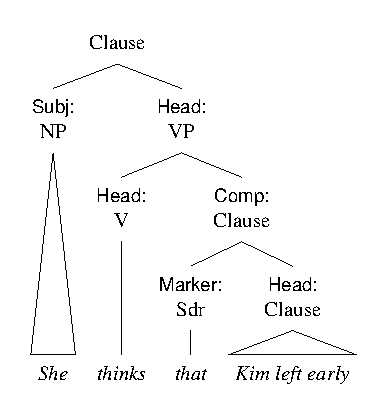
\includegraphics[width=0.55\linewidth]{figures/she thinks that kim left.pdf}
    \caption{Cây cú pháp cho thấy phụ thuộc hóa: \mention{that Kim left early} làm bổ ngữ trong \mention{She thinks that Kim left early}}\label{fig:sub-tree-sub-vi}
\end{figure}

Lưu ý rằng trong cấu trúc phụ thuộc, \mention{that} xuất hiện như một dấu hiệu. Nó không phóng chiếu cụm từ riêng mà chỉ báo điểm bắt đầu của mệnh đề phụ thuộc. \term{Dấu hiệu} (\term{marker}, Mk) là một loại thành phần phụ thuộc cho biết trung tâm của nó liên hệ về mặt ngữ pháp với cấu trúc lớn hơn như thế nào.

Mệnh đề nội dung có thể đảm nhiệm nhiều chức năng trong cấu trúc lớn hơn.

\ea \label{ex:content-funcs-vi}
    \ea \gll I suspect {\ob}that he left{\cb}.\\
        tôi nghi-PRS Sdr anh-ấy rời-đi-PST\\
    \glt \trans{Tôi nghi rằng anh ấy đã đi.} [trong VP]
    \ex \gll The fact {\ob}that he left{\cb} is clear.\\
        DEF sự-việc Sdr anh-ấy rời-đi-PST là-PRS rõ\\
    \glt \trans{Việc anh ấy đã đi là rõ ràng.} [trong NP]
    \ex \gll I'm glad {\ob}that he left{\cb}.\\
        tôi-là vui Sdr anh-ấy rời-đi-PST\\
    \glt \trans{Tôi vui vì anh ấy đã đi.} [trong AdjP]
    \ex \gll We can proceed provided {\ob}that he left{\cb}.\\
        chúng-ta có-thể-PRS tiếp-tục miễn-là Sdr anh-ấy rời-đi-PST\\
    \glt \trans{Chúng ta có thể tiếp tục miễn là anh ấy đã đi.} [trong PP]
    \ex \gll Whether or not he left is unclear.\\
        liệu hay không anh-ấy rời-đi-PST là-PRS không-rõ\\
    \glt \trans{Không rõ liệu anh ấy đã đi hay chưa.} [chủ ngữ]
    \ex \gll It's unclear whether or not he left.\\
        điều-đó-là không-rõ liệu hay không anh-ấy rời-đi-PST\\
    \glt \trans{Không rõ liệu anh ấy đã đi hay chưa.} [chủ ngữ ngoại vị]
    \z
\z

Trong mệnh đề nội dung trần thuật, dấu hiệu, tức từ phụ thuộc hóa \mention{that}, có thể bắt buộc, tùy chọn, hoặc không được phép, tùy chức năng của mệnh đề.

\ea\label{ex:marker-need-vi}
    \ea \gll That Kim left surprised no one.\\
        Sdr Kim rời-đi-PST làm-ngạc-nhiên-PST không ai\\
    \glt \trans{Việc Kim đi không làm ai ngạc nhiên.} [bắt buộc]
    \ex \gll I know that Kim left.\\
        tôi biết-PRS Sdr Kim rời-đi-PST\\
    \glt \trans{Tôi biết rằng Kim đã đi.} [tùy chọn]
    \ex \gll *We left before that Kim arrived.\\
        *chúng-tôi rời-đi-PST trước-khi Sdr Kim đến-PST\\
    \glt \trans{Nghĩa dự kiến: chúng tôi đã đi trước khi Kim đến. Trong tiếng Anh, \mention{that} không dùng được ở đây.} [*; không được phép]
\z
\z
Các mệnh đề làm chủ ngữ như (\ref{ex:marker-need-vi}a) luôn cần dấu hiệu. Khi làm bổ ngữ, mệnh đề trần thuật thường có thể có hoặc không có dấu hiệu, như trong (b). Ngoại lệ lớn là khi chúng làm bổ ngữ trong PP, như (c).

\label{sec:sub-interrog-vi}

Mệnh đề nội dung nghi vấn đáng chú ý vì cú pháp của chúng khác với nghi vấn ở mệnh đề chính. Nghi vấn cơ bản ở mệnh đề chính như \mention{Did she accept?} có thể nhận ra nhờ đảo chủ ngữ và trợ động từ. Ở phiên bản phụ thuộc, tính nghi vấn được đánh dấu bằng \mention{whether} hoặc \mention{if}.

\ea mệnh đề nghi vấn cơ bản\label{ex:int-sub-vi}
    \ea \gll Did she accept?\\
        AUX cô-ấy chấp-nhận\\
    \glt \trans{Cô ấy đã chấp nhận chưa?} [chính, có đảo]
    \ex \gll I wonder {\ob}whether she accepted{\cb}.\\
        tôi tự-hỏi-PRS liệu cô-ấy chấp-nhận-PST\\
    \glt \trans{Tôi tự hỏi liệu cô ấy đã chấp nhận chưa.} [phụ thuộc]
    \z
\z
\ea mệnh đề nghi vấn có tiêu điểm
    \ea \gll How did we get here?\\
        làm-sao AUX chúng-ta đến đây\\
    \glt \trans{Làm sao chúng ta đến được đây?} [chính, có đảo]
    \ex \gll I wonder {\ob}how we got here{\cb}.\\
        tôi tự-hỏi-PRS làm-sao chúng-ta đến-PST đây\\
    \glt \trans{Tôi tự hỏi chúng ta đã đến đây bằng cách nào.} [phụ thuộc]
    \z
\z
Điểm này khó đối với người học tiếng Anh. Người mới học thường không đảo gì cả, nên tạo sai câu hỏi ở mệnh đề chính. Người học có kinh nghiệm hơn, sau khi đã nắm được đảo, đôi khi áp dụng nó khắp nơi và làm sai cấu trúc của nghi vấn phụ thuộc. Phải đến trình độ cao hơn nhiều thì sự phân biệt này mới trở nên thoải mái.

Tuy vậy, khác biệt cấu trúc giữa nghi vấn ở mệnh đề chính và nghi vấn phụ thuộc đang dần yếu đi, khi hiện tượng đảo tiếp tục lan rộng chậm chạp. Trong văn viết, nghi vấn nội dung phụ thuộc có đảo vẫn hiếm, nhưng trong lời nói, các ví dụ như (\ref{ex:non-inverted-interrogative-vi}) đã trở nên khá thường gặp. Có lẽ vài trăm năm nữa đảo sẽ là chuẩn cho mọi nghi vấn và các dấu hiệu sẽ trở thành tùy chọn. Tôi sẽ không thức chờ chuyện đó.

\ea\label{ex:non-inverted-interrogative-vi}
\gll We need a story of {\ob}how did we get here{\cb}.\\
    chúng-ta cần-PRS một câu-chuyện về làm-sao AUX chúng-ta đến đây\\
\glt \trans{Chúng ta cần một câu chuyện về việc làm sao chúng ta đến được đây.}
\z
Nhưng trong tiếng Anh hiện nay, một dấu hiệu, thường là \mention{whether} hoặc \mention{if}, gần như luôn bắt buộc trong mệnh đề nội dung nghi vấn cơ bản. Nếu không có nó, trong phần lớn trường hợp sẽ không thể phân biệt mệnh đề này với một mệnh đề trần thuật không đánh dấu.

\subsubsection*{Cấu trúc mandative}

Một tiểu loại đặc biệt của cấu trúc phụ thuộc là \term{cấu trúc mandative} (\term{mandative construction}). Nó xuất hiện với các vị ngữ diễn đạt yêu cầu, mệnh lệnh, hoặc sự cần thiết.

\ea \label{ex:mandative-vi}
    \ea \gll It is essential {\ob}that he be there{\cb}.\\
        điều-đó là-PRS thiết-yếu Sdr anh-ấy ở-PLAIN đó\\
    \glt \trans{Điều thiết yếu là anh ấy phải có mặt ở đó.} [present subjunctive]
    \ex \gll It is essential {\ob}that he should be there{\cb}.\\
        điều-đó là-PRS thiết-yếu Sdr anh-ấy nên ở đó\\
    \glt \trans{Điều thiết yếu là anh ấy nên có mặt ở đó.} [should]
    \ex \gll It is essential {\ob}that he is there{\cb}.\\
        điều-đó là-PRS thiết-yếu Sdr anh-ấy ở-PRS đó\\
    \glt \trans{Điều thiết yếu là anh ấy có mặt ở đó.} [indicative]
    \z
\z
Trong \term{thức giả định hiện tại} (\term{present subjunctive}), động từ dùng dạng nguyên. Ở đây, \mention{subjunctive} không có nghĩa là câu nói về điều không thật hoặc phản sự thật. Trong tiếng Anh \mention{that he be there}, điểm quan trọng là \mention{be} xuất hiện ở dạng nguyên trong ngữ cảnh yêu cầu hoặc cần thiết. Dạng có \mention{should} phổ biến hơn, hoặc ít nhất từng phổ biến hơn, trong tiếng Anh Anh. Tiếng Anh Mỹ thường chuộng thức giả định hiện tại. Trong \term{indicative} (\term{indicative}), động từ dùng dạng chia thì thông thường.

Điều này cho thấy ngay trong mệnh đề phụ thuộc cũng có thể có khác biệt ý nghĩa tinh tế và khác biệt khu vực. Từ góc độ giảng dạy, nên lưu ý rằng dạng indicative đang phổ biến hơn, nhất là trong ngữ cảnh thân mật, nhưng thức giả định hiện tại vẫn là chuẩn trong văn viết trang trọng.

\begin{tblsframedsymbol}{Kiểm tra hiểu biết: mệnh đề bao chứa và mệnh đề phụ thuộc}{test}
Hãy nhận diện các quan hệ cấu trúc.
\begin{itemize}[noitemsep, leftmargin=*]
    \item Trong \mention{I know that she thinks that he left}, hãy xác định mệnh đề chính, các mệnh đề bao chứa, và các mệnh đề phụ thuộc.
    \item Giải thích vì sao \mention{She asked whether he left} không có đảo, còn \mention{Did he leave?} thì có.
    \item Tìm cấu trúc mandative: \mention{It's important that he be careful} và \mention{It's important that he is careful}.
\end{itemize}
Hiểu các quan hệ cấu trúc này giúp ta thấy rõ hơn ý nghĩa được tạo ra từ kiến trúc cú pháp như thế nào.
\end{tblsframedsymbol}

\subsection{Mệnh đề so sánh}

Kiểu mệnh đề phụ thuộc hữu hạn chính thứ hai là mệnh đề so sánh. Mệnh đề so sánh hoàn tất một phép so sánh, như trong (\ref{ex:comparative-intro-vi}).

\ea \label{ex:comparative-intro-vi}
    \ea \gll The ice was thicker than {\ob}we expected{\cb}.\\
        DEF băng là-PST dày-COMP hơn chúng-tôi mong-đợi-PST\\
    \glt \trans{Lớp băng dày hơn chúng tôi mong đợi.}
    \ex \gll She writes faster than {\ob}she speaks{\cb}.\\
        cô-ấy viết-PRS nhanh-COMP hơn cô-ấy nói-PRS\\
    \glt \trans{Cô ấy viết nhanh hơn nói.}
    \ex \gll It doesn't cost as much as {\ob}I'd thought{\cb}.\\
        nó NEG tốn-PRS bằng nhiều bằng tôi nghĩ-PST\\
    \glt \trans{Nó không đắt như tôi đã nghĩ.}
    \z
\z

Điểm phân biệt mệnh đề so sánh với mệnh đề nội dung là mệnh đề so sánh có ellipsis: một phần bị lược bỏ vì có thể khôi phục từ ngữ cảnh. Trong (\ref{ex:comparative-ellipsis-vi}), dấu ... chỉ phần bị lược.\footnote{Ở một chương trước, tôi đã giới thiệu gap. Gap là vị trí cấu trúc trong cây. Ellipsis là vật liệu có thể khôi phục về mặt nghĩa từ ngữ cảnh, nhưng không hiện diện như một yếu tố cú pháp.}

\ea \label{ex:comparative-ellipsis-vi}
    \ea \gll Kim read more books than {\ob}Pat read ...{\cb}.\\
        Kim đọc-PST nhiều-COMP sách-PL hơn Pat đọc-PST ...\\
    \glt \trans{Kim đọc nhiều sách hơn Pat đọc.}
    \ex \gll Kim read more books than {\ob}Pat did ...{\cb}.\\
        Kim đọc-PST nhiều-COMP sách-PL hơn Pat AUX.PST ...\\
    \glt \trans{Kim đọc nhiều sách hơn Pat.}
    \ex \gll Kim read more books than {\ob}Pat{\cb}.\\
        Kim đọc-PST nhiều-COMP sách-PL hơn Pat\\
    \glt \trans{Kim đọc nhiều sách hơn Pat.}
    \z
\z

Hai dạng đầu cho thấy ellipsis. Trong (b), VP pro-form \mention{did} được dùng thay vì lặp lại \mention{read}. Dạng thứ ba (c) có \mention{Pat} làm bổ ngữ NP chứ không phải bổ ngữ mệnh đề. Cả ba về cơ bản có cùng nghĩa.

Không giống phần lớn trường hợp ellipsis, trong mệnh đề so sánh, nếu nói rõ phần bị lược thì câu trở nên không chấp nhận được. Chẳng hạn, không nói *\mention{Kim read more books than Pat read 20 books} hoặc *\mention{It's not as deep as it is 20 cm wide}. Ellipsis là phần cốt lõi của kiểu mệnh đề này. Cấu trúc của mệnh đề so sánh được cho trong Figure~\ref{fig:comp-tree-vi}.

\begin{figure}
    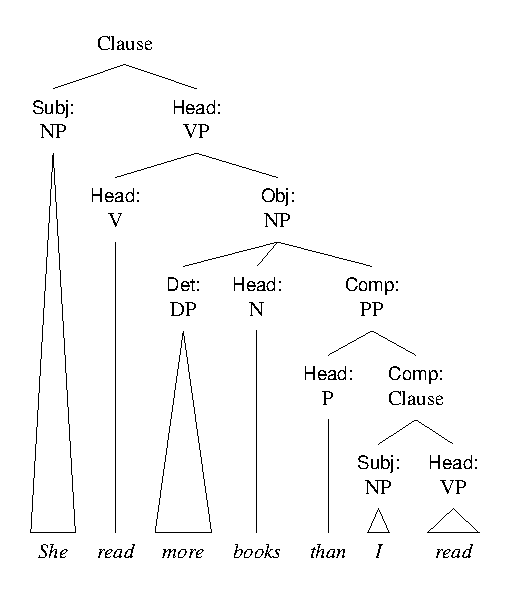
\includegraphics[width=0.7\linewidth]{figures/she read more books than I read.pdf}
    \caption{Cây cú pháp của mệnh đề so sánh có ellipsis}\label{fig:comp-tree-vi}
\end{figure}

Tùy loại so sánh, mệnh đề so sánh làm bổ ngữ trong PP có \mention{than} hoặc \mention{as}.

\ea \label{ex:comp-markers-vi}
    \ea \gll Kim is taller than {\ob}Pat is{\cb}.\\
        Kim là-PRS cao-COMP hơn Pat là-PRS\\
    \glt \trans{Kim cao hơn Pat.} [bất bình đẳng]
    \ex \gll Kim is as tall as {\ob}Pat is{\cb}.\\
        Kim là-PRS bằng cao bằng Pat là-PRS\\
    \glt \trans{Kim cao ít nhất bằng Pat.} [bình đẳng\footnote{Nhãn \mention{bình đẳng} ở đây có thể gây hiểu nhầm. Ví dụ này không có nghĩa là Kim và Pat cao đúng bằng nhau; nó có nghĩa là Kim không thấp hơn Pat, và Kim cũng có thể cao hơn.}]
    \z
\z
Trong (\ref{ex:comp-markers-vi}a), \mention{than} biểu thị bất bình đẳng; trong (b), \mention{as} đánh dấu bình đẳng. \mention{As} thứ nhất là trạng từ. Cụm \mention{as tall} là AdjP, trong đó \mention{as} làm thành phần bổ nghĩa. \mention{As} thứ hai là giới từ.

Người học tiếng Anh gặp vài khó khăn với mệnh đề so sánh.
\begin{itemize}[noitemsep]
    \item Biết phần nào, khi nào, và bao nhiêu phần có thể bị lược.
    \item Nắm các khuôn mẫu khác nhau cho bình đẳng và bất bình đẳng.
    \item Xử lý các phép so sánh phức tạp có nhiều thành tố liên quan.
\end{itemize}

Tin tốt là mệnh đề so sánh theo những khuôn mẫu khá đều. Trước khi xử lý các cấu trúc phức tạp hơn, người học thường có thể nắm các mẫu cơ bản như \mention{taller than} \trans{cao hơn ...} và \mention{as tall as} \trans{cao ít nhất bằng ...}.

\section{Phối hợp đẳng lập}\label{sec:coordination-vi}

Phụ thuộc hóa tạo ra quan hệ lệ thuộc giữa các mệnh đề; \term{phối hợp đẳng lập} nối các thành tố có cùng địa vị cú pháp. Ở trung tâm của hệ thống này là một lớp từ đóng rất nhỏ: \term{từ phối hợp đẳng lập} (\term{coordinator}, Crd). Các thành viên chính là \mention{and}, \mention{or}, và \mention{but}; cần cả ba chỉ để liệt kê đủ ba từ ấy. Giống từ phụ thuộc hóa, từ phối hợp đẳng lập cũng hoạt động như dấu hiệu.

Ở đây, \term{phối hợp đẳng lập} không chỉ có nghĩa là \mention{phối hợp} theo nghĩa làm việc nhịp nhàng hoặc sắp xếp hoạt động. Trong tiếng Việt, \mention{phối hợp} rất dễ gợi nghĩa tổ chức hoặc quản lý. Trong chương này, nghĩa là kỹ thuật: hai hay nhiều thành tố có cùng địa vị cú pháp, và không thành tố nào là trung tâm của toàn bộ cấu trúc. Nếu bỏ qua điểm này, người đọc dễ hiểu nhầm phối hợp đẳng lập thành việc nối ý lỏng lẻo hoặc lập danh sách đơn thuần.

Hãy xem các ví dụ sau.

\ea \label{ex:coord-basic-vi}
    \ea \gll {\ob}Jane is a good teacher{\cb} {\ob}and her students really like her{\cb}.\\
        Jane là-PRS một giỏi giáo-viên và của-cô-ấy sinh-viên-PL thật-sự thích-PRS cô-ấy\\
    \glt \trans{Jane là một giáo viên giỏi và sinh viên của cô ấy thật sự thích cô ấy.}
    \ex \gll They offered us a choice of {\ob}red wine{\cb}, {\ob}white wine{\cb}, {\ob}or beer{\cb}.\\
        họ đề-nghị-PST chúng-tôi một lựa-chọn của đỏ rượu trắng rượu hoặc bia\\
    \glt \trans{Họ cho chúng tôi lựa chọn giữa rượu vang đỏ, rượu vang trắng, hoặc bia.}
    \ex \gll Her assistant is {\ob}very young{\cb} {\ob}but a quick learner{\cb}.\\
        của-cô-ấy trợ-lý là-PRS rất trẻ nhưng một nhanh người-học\\
    \glt \trans{Trợ lý của cô ấy rất trẻ nhưng học rất nhanh.}
    \z
\z
Trong các ví dụ này, các phần liên quan hoạt động như \term{thành tố phối hợp} (\term{coordinate}). Chức năng này có thể được hiện thực bằng mệnh đề như trong (\ref{ex:coord-basic-vi}a), bằng NP hoặc các cụm từ khác như trong (b), và hiếm hơn, bằng sự pha trộn phạm trù như AdjP và NP trong (c). Từ phối hợp đẳng lập thường biểu đạt các quan hệ khác nhau: \mention{and} cho thêm vào, \mention{or} cho lựa chọn, và \mention{but} cho tương phản.

Điểm khác biệt lớn giữa phối hợp đẳng lập và các cấu trúc đã thấy trước đó là phối hợp đẳng lập không có trung tâm. Không thành tố phối hợp nào là trung tâm của toàn bộ cấu trúc. Điều này hiện rõ trong một phép thử đơn giản. Trong nhiều trường hợp, ta có thể thay toàn bộ cấu trúc phối hợp bằng một trong các thành tố phối hợp.

\ea \label{ex:coord-replace-vi}
    \ea \gll Her assistant is very young.\\
        của-cô-ấy trợ-lý là-PRS rất trẻ\\
    \glt \trans{Trợ lý của cô ấy rất trẻ.}
    \ex \gll Her assistant is a quick learner.\\
        của-cô-ấy trợ-lý là-PRS một nhanh người-học\\
    \glt \trans{Trợ lý của cô ấy học rất nhanh.}
    \z
\z
(\ref{ex:coord-replace-vi}a) và (b) đều là lựa chọn ngữ pháp thay cho (\ref{ex:coord-basic-vi}c). Điều này khác với cấu trúc có trung tâm như \mention{very young}. Trong trường hợp ấy, ta có thể dùng riêng trung tâm (\mention{she's young}), nhưng không dùng riêng thành phần phụ thuộc (*\mention{she's very}). Cấu trúc phối hợp được cho trong Figure~\ref{fig:coord-basic-vi}.

\begin{figure}
    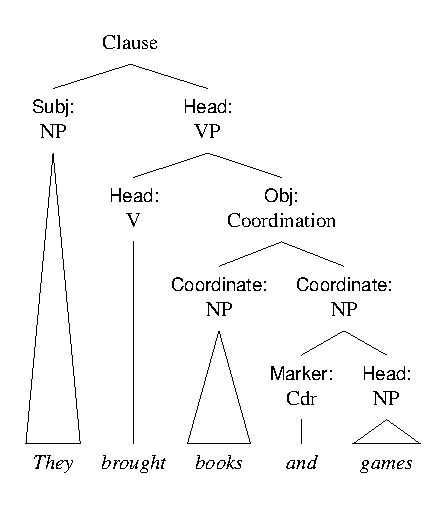
\includegraphics[width=0.65\linewidth]{figures/the brought books and games.pdf}
    \caption{Phối hợp đẳng lập cơ bản có dấu hiệu: \mention{They brought books and games}}\label{fig:coord-basic-vi}
\end{figure}

\subsection{Các thuộc tính của phối hợp đẳng lập}

Ba thuộc tính quan trọng phân biệt phối hợp đẳng lập với các cấu trúc khác.

Không có giới hạn ngữ pháp đối với số lượng thành tố phối hợp. \mention{But} là ngoại lệ.

\ea \label{ex:coord-multiple-vi}
\gll Nothing noble, sublime, profound, delicate, tasteful or even decent can find a place.\\
    không-gì cao-thượng trác-tuyệt sâu-sắc tinh-tế có-thẩm-mỹ hoặc thậm-chí đứng-đắn có-thể tìm một chỗ\\
\glt \trans{Không điều gì cao thượng, trác tuyệt, sâu sắc, tinh tế, có thẩm mỹ, hoặc thậm chí đứng đắn có thể có chỗ.}
\z

Các thành tố phối hợp phải tương tự về chức năng. Nếu dùng riêng, chúng phải có khả năng đảm nhiệm cùng một chức năng.

\ea \label{ex:coordinate-function-vi}
    \ea \gll I'll be back next week or at the end of the month.\\
        tôi-FUT có-mặt trở-lại kế tuần hoặc tại DEF cuối của DEF tháng\\
    \glt \trans{Tôi sẽ trở lại tuần tới hoặc vào cuối tháng.} [phụ ngữ thời gian]
    \ex \gll *We're leaving Rome and next week.\\
        *chúng-tôi-PRS rời Rome và tuần tới\\
    \glt \trans{Cấu trúc dự kiến: chúng tôi rời Rome và tuần tới. Câu này lạ trong tiếng Anh vì \mention{Rome} là object, còn \mention{next week} là adjunct.} [*; object và adjunct]
    \z
\z

Thành tố phối hợp mở rộng, tức thành tố phối hợp đi kèm từ phối hợp, không thể được đưa lên đầu.

\ea \label{ex:coord-front-vi}
    \ea \gll They attended but they aren't members.\\
        họ tham-dự-PST nhưng họ NEG-là-PRS thành-viên-PL\\
    \glt \trans{Họ đã tham dự, nhưng họ không phải là thành viên.}
    \ex \gll *But they aren't members, they attended.\\
        *nhưng họ NEG-là-PRS thành-viên-PL họ tham-dự-PST\\
    \glt \trans{Nghĩa dự kiến: họ đã tham dự, nhưng họ không phải là thành viên. Trong tiếng Anh, không thể đưa thành tố phối hợp mở rộng với \mention{but} lên đầu theo cách này.} [*]
    \z
\z

\subsection{Về từ phối hợp ở đầu câu}

Có một lời khuyên theo kiểu quy phạm rằng không nên bắt đầu câu bằng từ phối hợp như \mention{and} hoặc \mention{but}. Lệnh cấm này không có cơ sở trong ngữ pháp hay cách dùng tiếng Anh. Trong suốt lịch sử tiếng Anh, những người viết giỏi vẫn dùng từ phối hợp ở đầu câu. Bạn cũng sẽ thấy nhiều ví dụ trong chương này và trong các chương khác của sách.

Tuy nhiên, từ phối hợp ở đầu câu không thể buộc câu mới vào câu trước như một trường hợp phối hợp đẳng lập theo nghĩa cú pháp hẹp. Hãy nhớ hạn chế về fronting trong (\ref{ex:coord-front-vi}). Thay vào đó, nó có thể hoạt động như \term{từ nối diễn ngôn} (\term{discourse connector}), báo cho người đọc biết câu mới liên hệ với điều vừa nói như thế nào.

Đây là điểm người đọc tiếng Việt dễ hiểu nhầm. Trong tiếng Việt, bắt đầu câu bằng \mention{và}, \mention{nhưng}, \mention{tuy nhiên}, hoặc \mention{vì vậy} như từ nối diễn ngôn là rất tự nhiên. Nhưng phối hợp đẳng lập trong chương này là một quan hệ cú pháp bên trong một cấu trúc, trong đó các thành tố được nối có địa vị ngang nhau.

Giới hạn thật sự chỉ là phong cách: nếu lạm dụng từ nối đầu câu, văn sẽ đơn điệu; nếu dùng có cân nhắc, chúng giúp điều khiển dòng diễn ngôn.

\subsection{Các kiểu phối hợp đẳng lập}

Phân biệt đơn giản nhất là giữa \term{phối hợp đẳng lập đối xứng} (\term{symmetric coordination}) và \term{phối hợp đẳng lập không đối xứng} (\term{asymmetric coordination}). Trong phối hợp đối xứng, đảo thứ tự các thành tố phối hợp không làm đổi nghĩa; trong phối hợp không đối xứng, thứ tự có ảnh hưởng.

\ea \label{ex:coord-sym-vi}
    \ea \gll I was hungry and tired.\\
        tôi là-PST đói và mệt\\
    \glt \trans{Tôi đói và mệt.} [đối xứng]
    \ex \gll I got up and had breakfast.\\
        tôi thức-PST dậy và ăn-PST bữa-sáng\\
    \glt \trans{Tôi dậy và ăn sáng.} [không đối xứng]
    \z
\z
Trong (\ref{ex:coord-sym-vi}a), đảo thứ tự các thành tố phối hợp không đổi nghĩa. Nhưng trong (b), thứ tự gợi ra trình tự thời gian: việc dậy xảy ra trước bữa sáng.

Ta cũng phân biệt \term{phối hợp phân phối} (\term{distributive coordination}) và \term{phối hợp tập thể} (\term{joint coordination}).

\ea \label{ex:coord-dist-vi}
    \ea \gll Kim and Pat are fine players.\\
        Kim và Pat là-PRS giỏi cầu-thủ-PL\\
    \glt \trans{Kim và Pat là những cầu thủ giỏi.} [phân phối]
    \ex \gll Kim and Pat are a good pair.\\
        Kim và Pat là-PRS một tốt cặp\\
    \glt \trans{Kim và Pat là một cặp ăn ý.} [tập thể]
    \z
\z
Trong (\ref{ex:coord-dist-vi}a), phẩm chất cầu thủ giỏi áp dụng riêng cho Kim và cho Pat. Trong (b), phẩm chất là một cặp ăn ý chỉ áp dụng cho hai người cùng nhau; một người riêng lẻ không thể là một cặp.

\subsection{Đánh dấu phối hợp đẳng lập}

Phối hợp đẳng lập có thể được đánh dấu theo vài cách.
\begin{itemize}[noitemsep]
    \item bằng từ phối hợp: \mention{red and blue}
    \item không có dấu hiệu tường minh: \mention{red, white, blue}
    \item lặp từ phối hợp: \mention{red or white or blue}
    \item bằng các dấu hiệu tương liên: \mention{both red and blue}
\end{itemize}

Từ phối hợp thường biểu đạt thêm vào (\mention{and}), lựa chọn (\mention{or}), và tương phản (\mention{but}); nhưng trong phối hợp không đối xứng, chúng có thể mang thêm nghĩa.

\ea \label{ex:coord-meaning-vi}
    \ea \gll Pay within a week and you'll get a discount.\\
        trả-tiền trong-vòng một tuần và bạn-FUT nhận một giảm-giá\\
    \glt \trans{Nếu bạn trả tiền trong vòng một tuần, bạn sẽ được giảm giá.} [điều kiện]
    \ex \gll Pay within a week or you'll lose the discount.\\
        trả-tiền trong-vòng một tuần hoặc bạn-FUT mất DEF giảm-giá\\
    \glt \trans{Nếu bạn không trả tiền trong vòng một tuần, bạn sẽ mất khoản giảm giá.} [điều kiện phủ định]
    \z
\z

\begin{tblsframedsymbol}{Nhận diện khuôn mẫu: phối hợp hay phụ thuộc hóa?}{test}
Dùng các phép thử chẩn đoán để phân biệt các cấu trúc.
\begin{itemize}[noitemsep, leftmargin=*]
    \item Trong \mention{She thinks that he left} và \mention{She left and he stayed}: ví dụ nào đặt một mệnh đề vào trong mệnh đề khác, và ví dụ nào nối hai mệnh đề ngang hàng?
    \item Trong \mention{Although it rained, we went} và \mention{It rained but we went}: ví dụ nào cho thấy thứ bậc phụ thuộc, và ví dụ nào cho thấy địa vị ngang hàng?
    \item Trong \mention{*But we went, it rained} và \mention{Although it rained, we went}: fronting cho thấy gì về cấu trúc?
\end{itemize}
Các phép thử này giúp phân biệt lồng ghép theo thứ bậc với nối các thành tố ngang hàng.
\end{tblsframedsymbol}

Sau khi đã giới thiệu từ phối hợp, ta đã gặp tất cả các phạm trù từ vựng chính trong tiếng Anh, trừ thán từ. Ta cũng đã thấy những chức năng cú pháp chính mà chúng đảm nhiệm trong mệnh đề.

\subsection{Cấu trúc của phối hợp đẳng lập}

Khi ta phối hợp các thành tố, chúng phải chia sẻ cùng một chức năng cú pháp. Nghĩa là có thể phối hợp bổ ngữ với bổ ngữ, hoặc thành phần bổ nghĩa với thành phần bổ nghĩa, nhưng không thể phối hợp một bổ ngữ với một thành phần bổ nghĩa. Hãy so sánh.

\ea \label{ex:coord-function-vi}
    \ea \gll We listened {\ob}to the teacher{\cb} {\ob}and the students{\cb}.\\
        chúng-tôi nghe-PST với DEF giáo-viên và DEF sinh-viên-PL\\
    \glt \trans{Chúng tôi đã nghe giáo viên và các sinh viên.} [bổ ngữ]
    \ex \gll We listened {\ob}Monday{\cb} and {\ob}Tuesday{\cb}.\\
        chúng-tôi nghe-PST thứ-Hai và thứ-Ba\\
    \glt \trans{Chúng tôi đã nghe vào thứ Hai và thứ Ba.} [thành phần bổ nghĩa]
    \ex \gll *We listened {\ob}to the teachers{\cb} and {\ob}Monday{\cb}.\\
        *chúng-tôi nghe-PST với DEF giáo-viên-PL và thứ-Hai\\
    \glt \trans{Cấu trúc dự kiến nghe lạ trong tiếng Anh. \mention{to the teachers} là bổ ngữ, còn \mention{Monday} là thành phần bổ nghĩa.} [*; chức năng trộn lẫn]
    \z
\z
Các thành tố được phối hợp, tức \term{thành tố phối hợp}, có thể đến từ bất kỳ kiểu cụm lớn nào: danh từ, động từ, tính từ, giới từ, cụm lớn hơn, hoặc mệnh đề. Điều quan trọng là chúng hoạt động theo cùng một cách trong cấu trúc lớn hơn.

\subsection{Phối hợp có và không có dấu hiệu}

Phối hợp đẳng lập có thể có từ phối hợp tường minh, hoặc không có. Khi không có từ phối hợp, ta gọi đó là \term{phối hợp không có từ phối hợp} (\term{asyndetic coordination}).

\ea \label{ex:coord-marking-vi}
    \ea \gll She brought {\ob}games{\cb}, {\ob}stories{\cb}, {\ob}songs{\cb}.\\
        cô-ấy mang-PST trò-chơi-PL truyện-PL bài-hát-PL\\
    \glt \trans{Cô ấy mang trò chơi, truyện, và bài hát.} [không có từ phối hợp]
    \ex \gll She brought {\ob}games{\cb}, {\ob}stories{\cb}, and {\ob}songs{\cb}.\\
        cô-ấy mang-PST trò-chơi-PL truyện-PL và bài-hát-PL\\
    \glt \trans{Cô ấy mang trò chơi, truyện, và bài hát.} [có từ phối hợp]
    \z
\z
Bên cạnh phối hợp đơn giản với một từ phối hợp, ta còn có \term{phối hợp tương liên} (\term{correlative coordination}). Ở đây, dấu hiệu xuất hiện với nhiều hơn một thành tố phối hợp.

\ea \label{ex:coord-correlative-vi}
    \ea \gll {\ob}Both{\cb} tired {\ob}and{\cb} hungry\\
        vừa mệt vừa đói\\
    \glt \trans{vừa mệt vừa đói}
    \ex \gll {\ob}Either{\cb} now {\ob}or{\cb} never\\
        hoặc bây-giờ hoặc không-bao-giờ\\
    \glt \trans{hoặc bây giờ, hoặc không bao giờ}
    \ex \gll {\ob}Neither{\cb} simple {\ob}nor{\cb} easy\\
        không đơn-giản cũng-không dễ\\
    \glt \trans{không đơn giản và cũng không dễ}
    \z
\z

\subsection{Phối hợp nhiều tầng}

Bản thân thành tố phối hợp có thể chứa phối hợp. Ta có thể gọi đó là phối hợp nhiều tầng. Hãy xét ví dụ sau.

\ea \label{ex:coord-layered-vi}
\gll The story was {\ob}short and sweet{\cb} but {\ob}complex and thought-provoking{\cb}.\\
    DEF câu-chuyện là-PST ngắn và ngọt-ngào nhưng phức-tạp và gợi-suy-nghĩ\\
\glt \trans{Câu chuyện ngắn gọn và dễ mến, nhưng phức tạp và gợi suy nghĩ.}
\z
Ở đây, có hai thành tố phối hợp chính được nối bằng \mention{but}. Nhưng mỗi thành tố ấy lại chứa phối hợp nội bộ với \mention{and}. Việc xếp tầng như vậy cho phép ta diễn đạt những quan hệ ý nghĩa phức tạp mà vẫn giữ cấu trúc rõ ràng. Cấu trúc nhiều tầng được cho trong Figure~\ref{fig:coord-layered-vi}.

\begin{figure}
    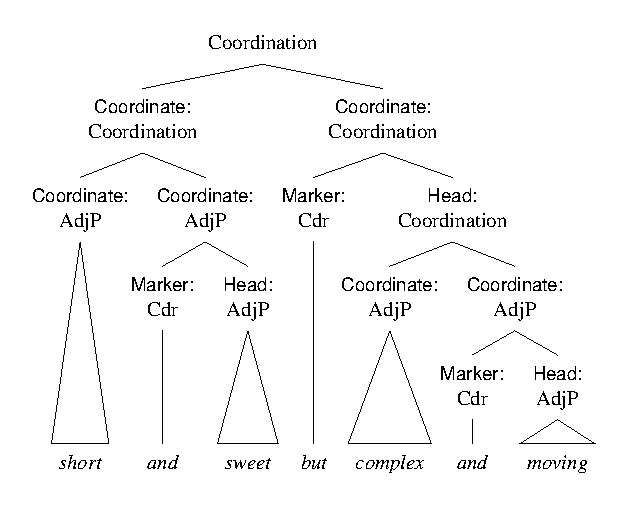
\includegraphics[width=0.9\linewidth]{figures/short and sweet but complex and moving.pdf}
    \caption{Phối hợp nhiều tầng: \mention{short and sweet but complex and moving}}\label{fig:coord-layered-vi}
\end{figure}

\subsection{Kiểu phối hợp đặc biệt}

Một kiểu phối hợp đặc biệt thú vị xuất hiện trong các cấu trúc so sánh.

\ea \label{ex:coord-comp-vi}
    \ea \gll He's as tall as {\ob}or taller than{\cb} his brother.\\
        anh-ấy-là bằng cao bằng hoặc cao-COMP hơn của-mình anh-em\\
    \glt \trans{Anh ấy cao ít nhất bằng anh/em trai mình, hoặc còn cao hơn.}
    \ex \gll She writes more {\ob}but understands less{\cb} than before.\\
        cô-ấy viết-PRS nhiều-COMP nhưng hiểu-PRS ít-COMP hơn trước\\
    \glt \trans{Cô ấy viết nhiều hơn trước, nhưng hiểu ít hơn.}
    \z
\z
Trong những cấu trúc này, quan hệ giữa các thành tố phối hợp và phần chúng chia sẻ thường phức tạp. Việc diễn giải chúng đòi hỏi hiểu cả phối hợp đẳng lập lẫn quan hệ so sánh.

\begin{tblsframedsymbol}{Tự kiểm tra nhanh: cấu trúc phức tạp}{test}
Thử phân tích các cấu trúc nhiều tầng.
\begin{itemize}[noitemsep, leftmargin=*]
    \item Trong \mention{I know that she left and he stayed}, hãy tìm tất cả các quan hệ phụ thuộc hóa và phối hợp.
    \item Trong \mention{Both young and talented, she succeeded}, hãy tìm các dấu hiệu tương liên và các tính từ được phối hợp.
    \item Phân tích cấu trúc này: \mention{He's taller than I thought but shorter than his brother}.
\end{itemize}
Khi hiểu các khuôn mẫu phức tạp này, ta thấy rõ phụ thuộc hóa và phối hợp đẳng lập cùng xây dựng ý nghĩa như thế nào.
\end{tblsframedsymbol}

\section{Tóm tắt}

Phụ thuộc hóa và phối hợp đẳng lập làm cùng một việc, nối các ý, nhưng bằng hai kiến trúc đối lập. Phụ thuộc hóa lồng một cấu trúc vào cấu trúc khác; phối hợp đẳng lập đặt các thành tố cạnh nhau. Lối viết tốt cân bằng cả hai. Khi ta nhận ra người học đang cố xây dựng cấu trúc nào và cấu trúc ấy vỡ ở đâu, ta không chỉ dừng lại ở cảm giác rằng có gì đó lạ; ta có thể gọi tên vấn đề: quá nhiều tầng, quá nhiều liệt kê, hoặc dùng từ phụ thuộc hóa ở nơi một từ phối hợp đã đủ.

\end{document}
